
\chapter{Sprint 4}
\label{Sprint4}
\lhead{Chapter 10. \emph{Sprint 4}}

\section{Duration}
The duration of the sprint was the following:
\begin{itemize}
\item Start: October, 21st
\item End: November, 03rd
\end{itemize}

\section{Planning}

The plan for this sprint consisted in one last development effort to complete the second product prototype before our meeting with the customer and in view of the feature freeze deadline.

Although some refactoring done last sprint did result in a slight improvement to the codebase, most of it did not make it into the master branch.
The reason for this was because we did not have enough spare resources to dedicate to this task, or we would have rather used those for report writing which was becoming an increasingly pressing task.

Regarding the collaboration with our colleague in Oslo, we discussed his contribution to the project during last sprint in an internal meeting.
We understood that it would have helped to be specific about what parts of the report we expected him to write. 
We also made a more realistic estimate of the amount of time he could dedicate the project being a full-time worker.
After these considerations, we planned less work for him for this sprint.
We were explicit about what parts of the report he should have worked on and encouraged him to track his time appropriately.
We tried to make him feel part of the team and we counted on him.

\section{Goal(s)}

The main goal of this sprint was to finalize and demonstrate a second prototype of the product, which included: 

\begin{itemize}
\item a) the back-end
\item b) the front-end
\item c) two Android application
\end{itemize}
These had to be ready for October the 24th when our customer planned to visit Trondheim.

\section{Results and feedback}

During this sprint we worked mostly on development, which proceeded without major issues.
A second prototype of the product was completed on schedule before our planned meeting with the customer, which would have been on the 24th.
However, the customer cancelled the meeting and proposed to reschedule it for the 30th.

Considering we had some more time to dedicate to development activities and in view of the feature freeze deadline (M3) by the end of the sprint, we took initiative and submitted a new possible application prototype idea to the customer.
It consisted of a web application which would feature HealthVault integration similarly to the Android application.
The customer expressed his interest in it because it would have used a different technology other than Android. He inquired about its feasibility in such a short amount of time (less than two weeks). We were confident that we could have re-used some code shipped with HealthVault SDK to minimize the amount of code we would have had to write ourselves, so we committed its development.

On the 30th of November, very early in the morning the customer sent us a mail were he cancelled our meeting. 
However, he was available for a Skype meeting.
We were able to demonstrate him our product via Skype, including the last application which had been developed in one week time. He was very pleased with our work.
We discussed with him about our presentation and agreed to have an additional presentation with the customer's colleagues after the 21st of November.

\section{Evaluation}

\begin{figure}
\centering
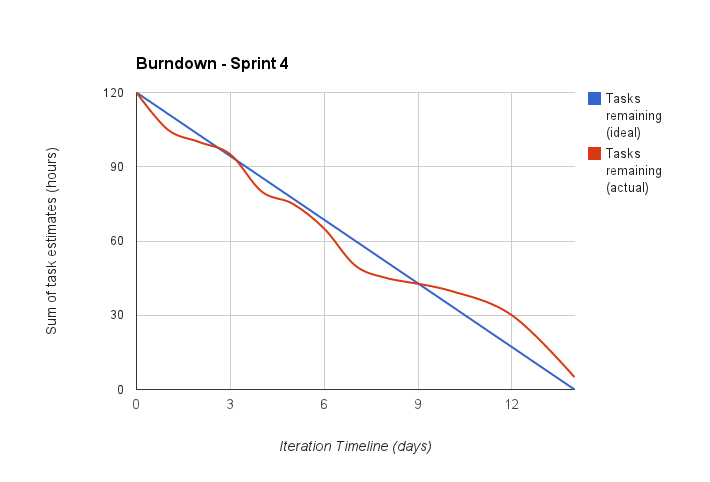
\includegraphics[scale=0.60]{../Figures/burndownSprint4.png}
\caption{Iteration burndown chart}
\label{figure:burndownsprint4}
\end{figure}

The sprint was very rewarding.
Receiving a good evaluation from the customer proved to be very valuable for the group, especially because the project was drawing to an end and timing was becoming tight.
There was no time left to make any big adjustments to the product.
The feedback from the customer motivated the group to keep up the good work and make one big final effort to finish the documentation and prepare a presentation.

We encountered a small problem during development regarding Withings integration with HealthVault, which we planned to use for our demonstration. 
Withings failed to send the data acquired by the scale device to HealthVault. 
Unfortunately, after various attempts, we were unable to solve the problem because we had no control over it.
Although the scenario for the demonstration had changed and did not include the Withings scale device any more, the functionality of the application itself had not, so we consider this a minor issue.

Regarding our collaboration with our colleague in Oslo, he appreciated our understanding of his situation and our attempts to plan a more appropriate amount of work for him. 
He managed to contribute more effectively during this sprint.

This iteration burndown chart is shown in figure \ref{figure:burndownsprint4}.
\clearpage
\section{Backlog}
See below the sprint backlog:
\begin{enumerate}[1.]
\item \textbf{Project management} included:
	\begin{itemize}
		\item \textbf{Sprint startup meeting}:
			included sprint planning and review
		\item \textbf{Weekly meetings}: 
			meetings with both the customer and the supervisor. Internal meeting with our colleague in Oslo
		\item \textbf{Meeting notes}:
			taking notes during meetings, reviewing of the notes
		\item \textbf{Status reports}:
			for both week 43 and 44
		\item \textbf{Risk analysis}:
			updated on a weekly basis
	\end{itemize}
	\item \textbf{System development}
		additional system development to accommodate fixes to the front end
	\item \textbf{Web application development}
		develop a web application which integrates weight measurements
		on HealthVault in our system
	\item \textbf{Report work}
		to be done by the team member in Trondheim
	\item \textbf{Additional report work}
		to be done by the team member in Oslo
	\item \textbf{Testing}
		perform unit and integration testing
\end{enumerate}

